\documentclass[10pt]{book}
\usepackage{sinhala}

\title{\bf ශුද්ධ වූ බයිබලය}
\author{ශුද්ධ වූ සභාව}

\newcommand{\uu}[1]{$^{#1}$}
\def\dummy{\uu{24}දෙවියන්වහන්සේ ඒ {\lq\lq}යහපත්{\rq\rq} බව දුටුසේක. \uu{25}දතවද දෙවියන්වහන්සේ: අපගේ {\bf ස්වරූපයෙන්} අපගේ සමානත්වය ලෙස මනුෂ්‍යයා සාදම්හ; ඔව්හු මුහුදේ මත්ස්‍යයන් කෙරෙහිද ආකාශයේ පක්ෂීන් කෙරෙහිද තිරිසනුන් කෙරෙහිද මුළු පොළොව කෙරෙහිද පොළොව පිට බඩගා යන සියල්ලන් කෙරෙහිද ආණ්ඩුකෙරෙත්වයි කීසේක. \uu{26}දදදෙවියන්වහන්සේ තමන් ස්වරූපයෙන් මනුෂ්‍යයා මැවුසේක, දෙවියන්වහන්සේගේ ස්වරූපයෙන් ඔහු මැවුසේක; පුරුෂයාද ස්ත්‍රියද කොට ඔවුන් මැවූසේක. \uu{27}දදියන්වහන්සේ ඔවුන්ට ආශීර්වාදකළසේක;}                           

\begin{document}                        
\frontmatter                            
\maketitle                              
\tableofcontents                        
\listoffigures
\listoftables
\mainmatter  

\part{පැරණි ගිවිසුම}                   
\chapter{උත්පත්ති}                
\dummy
 
\section{මැවීම}                  
\dummy

\subsection{කරුණාව}
\dummy

\subsubsection{ධෛර්යය}
\dummy
 
\paragraph{දේව භක්තිය} 
  \textsf{\dummy}\\
  {\textsf{පිරික්සුම} පිරික්සුම}

\begin{center}
\begin{tikzpicture}
    \begin{axis}[domain=0:1,
    xlabel=$\epsilon~~\text{ වෙනස}$,
    ylabel=$d(\epsilon)~~\text{ පරතරය}$,
    xtick={0,1},
	xticklabels={$0$, $1$},
	ytick={0,sqrt(6)/3},
	yticklabels={$0$, $\sqrt6/3$},
	grid=both]
    \addplot[mark=none, samples=100, red] function {sqrt(6)*(1-x)/3};
    \end{axis}
\end{tikzpicture}
\captionof{figure}{මුළු පොළෝතලයෙහි ඇති බීජ}
\end{center}
 
\dummy

\begin{equation}
\nabla c=\left({\partial c\over \partial a}, {\partial c\over \partial b}\right)=\left({1\over 2}\sqrt{b\over a},{1\over 2}\sqrt{a\over b}\right)
\end{equation}

\dummy
 
\part{අලුත් ගිවිසුම}           
\chapter{මතෙව්}                
\dummy


\begin{table}[!hbt]
\begin{center}
\caption{රූපය~\ref{fig:graph} හි අදෘශ්‍යමාන සංකූලතා}
\label{tab:data}
\begin{tabular}{|l|c|r|}
\hline
උස &  පළල & දිග \\
\hline
-5 & -5.39 & -5.42\\
-4 & -5.8 & -5.78\\
-3 & -6.25 & -6.21\\
-2 & -6.7 & -6.71\\
-1 & -7.28 & -7.3\\
\hline
\end{tabular}
\end{center}
\end{table}

\dummy
 
\section{නත්තල}                
\dummy

\subsection{ප්‍රඥාව}
\dummy

\subsubsection{දැනමිතිකම}
\dummy
 
\paragraph{දැනගැන්ම} 
\dummy


 
\dummy

\begin{center}
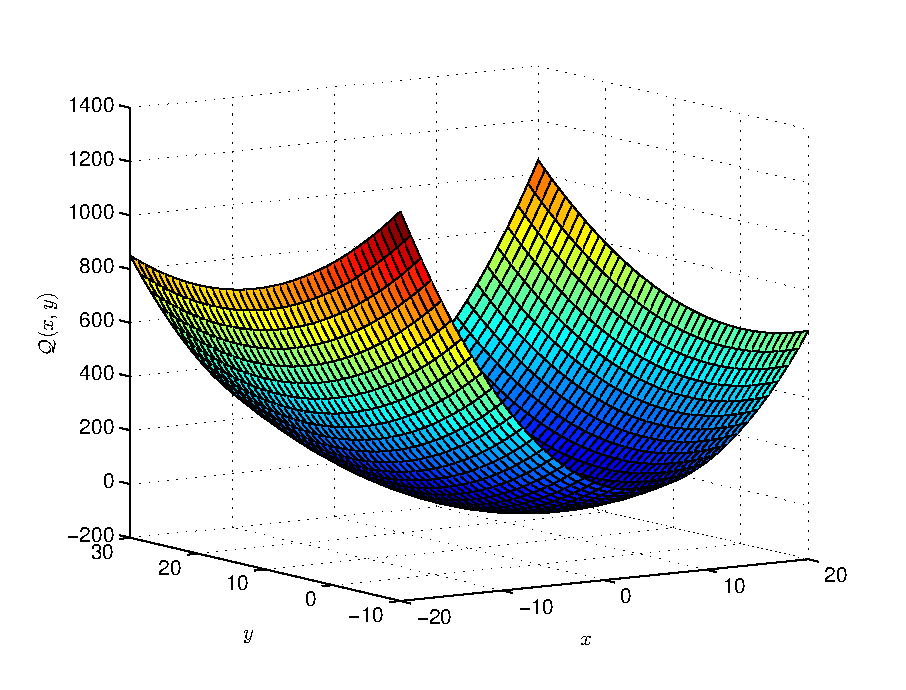
\includegraphics[scale=.7]{images/q-plot.eps}
\captionof{figure}{අභ්‍යාන්තරික සාන්දර්භය}
\label{fig:graph}
\end{center}

\dummy

 
\end{document}  